\chapter{Teaching Your PI Controller to Behave (Part VII)}

So far we have discussed the PI tuning problem in the context of a linear system.  This is because under steady-state conditions when the system transients settle out, you will probably be operating in the linear region, and \textit{that’s} when your feedback loop will either oscillate or not.  Therefore, performing a small-signal (linear) analysis will tell you how stable your system will be when it is not saturated.  But in most real-life scenarios, the system \textit{will} saturate because of limits on your voltage and/or current, especially under large transient conditions.  This saturation effect can play some real mind games with your PI controller; especially the integrator.  Since the maximum torque your motor can produce is determined by your current limit, the acceleration of the system is also limited.  But the integrator in the PI speed controller doesn’t know this, and it thinks it can make the motor speed up even faster by increasing its output.  This increased integrator output can’t help the situation since the system is already saturated.  All it does is create a very large output that will cause the system to overshoot when it \textit{does} come out of saturation.  For this reason, most PI integrators employ techniques to keep them from needlessly integrating while the system is saturated.

One technique which is commonly used is \textit{integrator clamping}, which establishes limits for the maximum and minimum values that the integrator output can have.  An example of this is illustrated in Figure \ref{fig:07_01}.  The most common scenario is to set the clamp values to be equal to the PI output limit values.  However, there is nothing that says that the integrator limits must \textit{equal} the PI output limits, and many designs use different clamp values based on the specific application.  As you might expect, the tighter you set the clamp limits, the less windup you will have to deal with when the system finally does come out of saturation.

\begin{figure}[H]
    \centering
    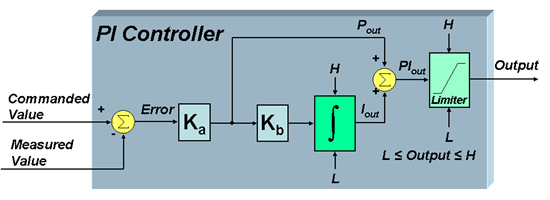
\includegraphics[width=1\linewidth]{07/01}
    \caption{PI Controller with Static Integrator Clamping}
    \label{fig:07_01}
\end{figure}

However, a more robust clamping scheme is shown in Figure \ref{fig:07_02}.  The thinking behind \textit{dynamic integrator clamping} is based on the rationale that if the system is already saturated by the P gain output, then why allow the integrator to continue integrating since it can’t help anyway.  Only during conditions where changes in the integrator output would affect changes in the PI controller output is the integrator allowed to integrate the error signal.


\begin{figure}[H]
    \centering
    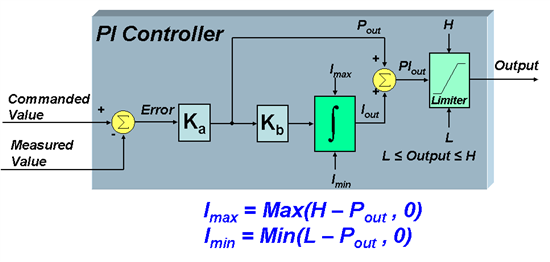
\includegraphics[width=1\linewidth]{07/02}
    \caption{PI Controller with Dynamic Integrator Clamping}
    \label{fig:07_02}
\end{figure}

The effectiveness of integrator clamping can be seen by the simulated velocity responses in Figure \ref{fig:07_03}.  The system is instantly stimulated with a commanded velocity step from zero to a target speed of \qty{1500}{\rpm}, which will obviously cause saturation.  Shown are the effects of system overshoot with \textit{no} clamping, \textit{static} clamping where the integrator clamp values equal the output clamp values, and finally \textit{dynamic} clamping.  As you can see, no integrator clamping at all is unacceptable as it results in horrendous overshoot which triggers further system saturation and oscillation.  Static integrator clamping dramatically improves the system response.  However, dynamic clamping improves performance even further, resulting in six times less overshoot than static clamping in this particular example.  An important but somewhat obvious point to remember about integrator clamping is that it only improves the overshoot response if the clamp activates.  If the commanded stimulation is small enough to keep the system in the linear mode of operation, then the overshoot you get will be determined exclusively by the damping factor.

\begin{figure}[H]
    \centering
    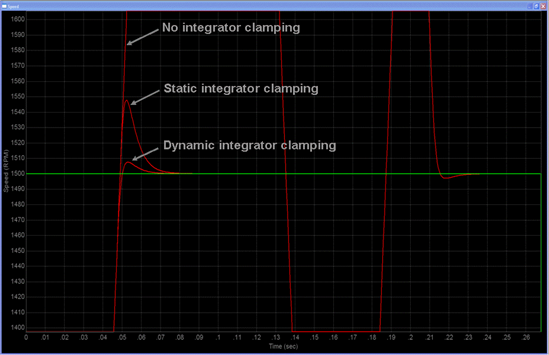
\includegraphics[width=1\linewidth]{07/03}
    \caption{Example Comparison of Integrator Clamping Techniques}
    \label{fig:07_03}
\end{figure}

Another technique that has been used to mitigate windup is \textit{integrator switching}.  With this technique, the integrator is only turned on at the \textit{end} of a commanded profile transition, or when the system output has pulled to within a specified range of the commanded input.  In the latter case, the output loading must be small (or at least somewhat predictable) in order to select a meaningful threshold for when to turn the integrator on.  But you must also be careful how and when you turn the integrator \textit{off}.  If you also reset the integrator output to zero when you switch it off, you can end up with a large and undesirable discontinuity in the output waveform if the integrator output was very large at the time.  But not resetting the output to zero can also have undesirable consequences when the integrator is turned back on.  For example, if the steady-state integrator output eventually changes polarity when it is turned back on again, the settling time will take much longer than if the integrator output had been reset.  My opinion about integrator switching is that it can be an effective technique to minimize windup, but getting good results can be tricky, and it is very much application dependent.

In my next blog, I want to double back and talk some more about PI tuning.  Now that we know how to put the puzzle together, the obvious question to ask is, “do we have all the pieces?”  Up until now, I have assumed the answer is \textit{yes}.  But there is one piece that all the other pieces fit around that we haven’t really talked a lot about, and that is \textbf{inertia}.  While this parameter is sometimes provided on a motor data sheet, it is almost never provided for the load you are driving.  Without it, you can’t accurately tune your velocity loop unless you rely heavily on trial and error.  In my next blog, I want to introduce you to TI’s new InstaSPIN-FOC algorithm, and propose a technique for how it can be used to actually \textit{measure} system inertia.  You don’t want to miss this one!  Until then\dots\\

Keep Those Motors Spinning,\\

\includegraphics[width=0.2\linewidth]{01/04_dave}
\vfill
\textit{Apr 13 2013 15:56 PM}